\documentclass[12pt]{article}
\usepackage[margin=2cm]{geometry}

\usepackage{graphicx}
\usepackage{amsmath}
\usepackage{booktabs}
\usepackage{multirow}
\usepackage{algorithm}
\usepackage{algpseudocode}
\usepackage{caption}
\usepackage{float}

\usepackage{pgfplots}
\pgfplotsset{compat=1.18}

\usepackage{listings}
\usepackage{xcolor}
\lstset{
    backgroundcolor=\color[HTML]{EEEEEE},
    commentstyle=\color[HTML]{6A9955},
    keywordstyle=\color[HTML]{0000FF},
    stringstyle=\color[HTML]{DD3300},
    basicstyle=\ttfamily\footnotesize,
    breakatwhitespace=false,
    breaklines=true,
    captionpos=t,
    keepspaces=true,
    numbers=none,
    numbersep=5pt,
    numberstyle=\tiny\color[rgb]{0.5,0.5,0.5},
    showspaces=false,
    showstringspaces=false,
    showtabs=false,
    tabsize=4,
    frame=single,
    escapeinside={<@}{@>}
}

\usepackage{xeCJK}
\setmainfont{Times New Roman}
\setCJKmainfont[AutoFakeBold=true,AutoFakeSlant=true]{TW-Kai}

\usepackage{indentfirst}
\setlength{\parindent}{0em}

\PassOptionsToPackage{hyphens}{url}\usepackage[hidelinks]{hyperref}
\newcommand{\algorithmautorefname}{Algorithm}
\newcommand*{\fullref}[1]{\hyperref[{#1}]{\ref*{#1} \nameref*{#1}}}

\begin{document}

\title{Logic Synthesis and Verification \\ PA3 Reinforcement Learning for Logic Synthesis Library Tuning for Technology Mapping}
\author{B11107051 李品翰}
\date{}
\maketitle

\section*{Assignment 1 (30\%): Environment setup and baseline replication}

\begin{figure}[H]
  \centering
  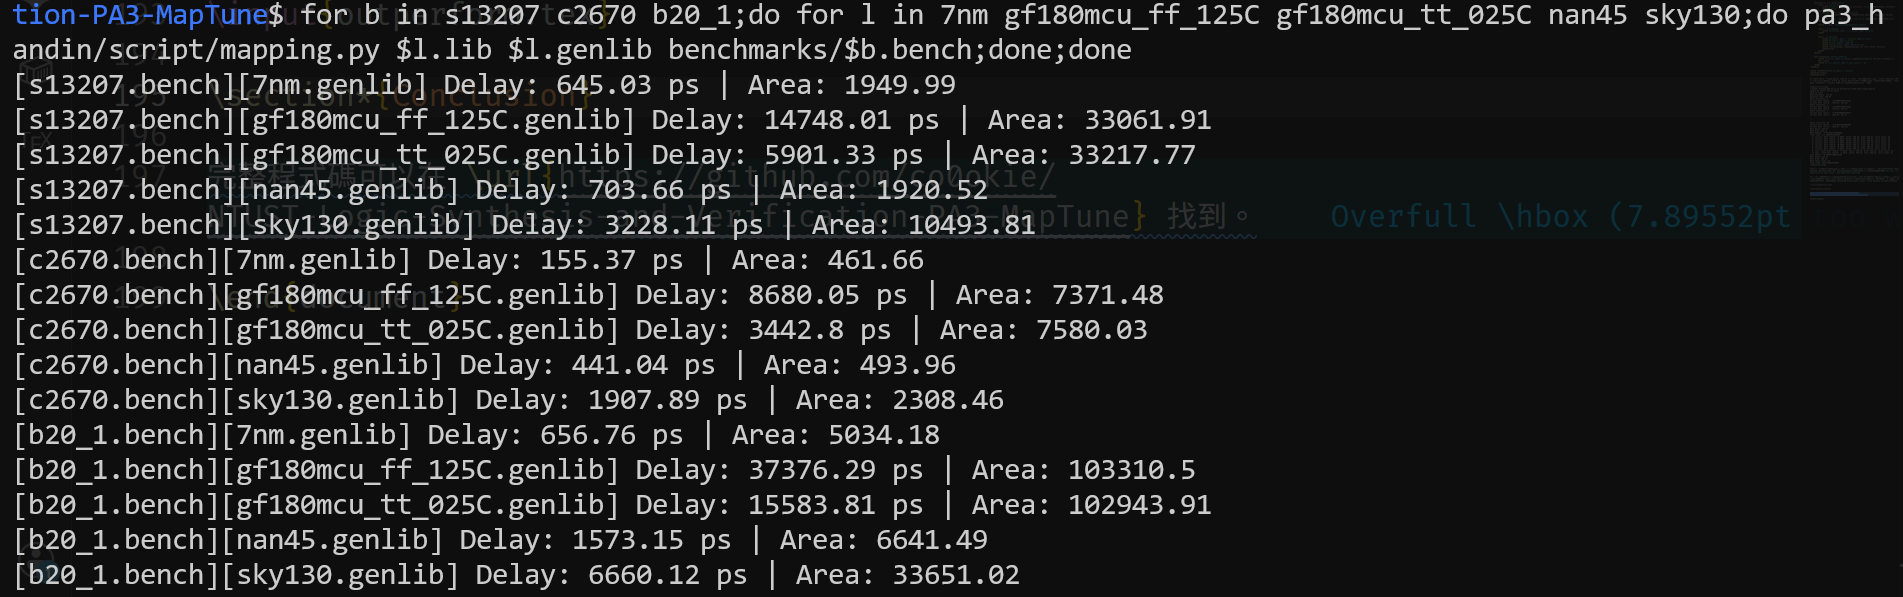
\includegraphics[width=\linewidth]{screenshot_a1.png}
\end{figure}

\begin{table}[H]
\centering
\caption{Baseline Technology Mapping Results}
\begin{tabular}{llrr}
\toprule
\textbf{Benchmark} & \textbf{Library} & \textbf{Delay (ps)} & \textbf{Area ($\mu m^2$)} \\
\midrule
\multirow{5}{*}{s13207} 
 & 7nm & 645.03 & 1949.99 \\
 & gf180mcu\_ff\_125C & 14748.01 & 33061.91 \\
 & gf180mcu\_tt\_025C & 5901.33 & 33217.77 \\
 & nan45 & 703.66 & 1920.52 \\
 & sky130 & 3228.11 & 10493.81 \\
\midrule
\multirow{5}{*}{c2670} 
 & 7nm & 155.37 & 461.66 \\
 & gf180mcu\_ff\_125C & 8680.05 & 7371.48 \\
 & gf180mcu\_tt\_025C & 3442.80 & 7580.03 \\
 & nan45 & 441.04 & 493.96 \\
 & sky130 & 1907.89 & 2308.46 \\
\midrule
\multirow{5}{*}{b20\_1} 
 & 7nm & 656.76 & 5034.18 \\
 & gf180mcu\_ff\_125C & 37376.29 & 103310.50 \\
 & gf180mcu\_tt\_025C & 15583.81 & 102943.91 \\
 & nan45 & 1573.15 & 6641.49 \\
 & sky130 & 6660.12 & 33651.02 \\
\bottomrule
\end{tabular}
\end{table}

\section*{Assignment 2 (30\%): Randomly sampling replication}

從 \autoref{fig:random_sample} 可以看出，即便只取 75 \~{} 150 個 cells (藍色部分)，仍然可能得到相當不錯的解，證明了 partial library 仍有機會贏過 full library。

% 請在 preamble 加入: \usepackage{pgfplots}
% \pgfplotsset{compat=1.18}
\begin{figure}[H]
\centering
\begin{minipage}{0.32\textwidth}
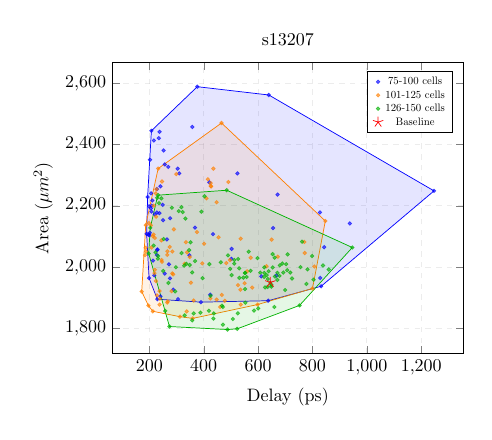
\begin{tikzpicture}[scale=0.65]
\begin{axis}[
    title={s13207},
    xlabel={Delay (ps)},
    ylabel={Area ($\mu m^2$)},
    legend pos=north east,
    legend style={nodes={scale=0.6, transform shape}},
    grid=both,
    grid style={dashed, opacity=0.3}
]
  \addplot [color=blue, fill=blue, fill opacity=0.1, forget plot] coordinates { (376.49, 2588.24) (207.68, 2444.31) (193.85, 2228.52) (190.21, 2108.15) (199.17, 1963.75) (229.57, 1894.93) (389.82, 1885.37) (637.14, 1890.03) (831.87, 1937.16) (1246.99, 2248.35) (639.41, 2561.18) (376.49, 2588.24) };
  \addplot [color=orange, fill=orange, fill opacity=0.1, forget plot] coordinates { (847.31, 2150.14) (465.62, 2469.74) (232.59, 2321.14) (186.87, 2136.61) (172.16, 1919.89) (196.69, 1874.17) (213.00, 1855.51) (312.59, 1838.01) (359.74, 1832.41) (598.01, 1877.44) (800.11, 1929.93) (847.31, 2150.14) };
  \addplot [color=green!70!black, fill=green!70!black, fill opacity=0.1, forget plot] coordinates { (946.59, 2063.59) (484.64, 2250.45) (232.54, 2234.36) (228.98, 2225.72) (203.51, 2127.51) (197.77, 2044.00) (274.22, 1805.82) (487.66, 1796.02) (523.34, 1798.36) (752.39, 1874.64) (946.59, 2063.59) };
  \addplot [only marks, mark=*, mark size=1pt, color=blue, opacity=0.6] coordinates { (228.16, 2038.87) (230.33, 2057.30) (241.03, 1904.50) (256.99, 2334.67) (502.81, 2059.16) (201.98, 2111.65) (206.32, 2240.42) (1246.99, 2248.35) (347.39, 2038.40) (368.27, 2128.45) (220.26, 2171.60) (358.20, 2456.91) (206.34, 2191.43) (376.49, 2588.24) (228.20, 2177.67) (304.36, 2320.90) (252.54, 2380.16) (421.09, 2276.11) (190.21, 2108.15) (211.33, 2216.86) (228.20, 2254.42) (193.85, 2228.52) (249.33, 2202.86) (831.87, 1937.16) (199.23, 2197.96) (654.98, 2127.05) (229.57, 1894.93) (272.37, 2008.77) (612.04, 1969.58) (524.07, 2305.27) (202.54, 2349.83) (237.63, 2441.04) (389.82, 1885.37) (250.55, 2152.71) (241.19, 2263.28) (305.72, 1895.17) (827.42, 2177.90) (269.74, 2326.73) (843.11, 2064.53) (639.41, 2561.18) (208.18, 2180.70) (199.17, 1963.75) (276.62, 2159.01) (213.75, 2020.90) (937.35, 2141.98) (228.73, 2055.20) (434.24, 2107.45) (216.86, 2412.81) (237.37, 2175.57) (637.14, 1890.03) (208.92, 2200.30) (234.96, 2420.28) (200.51, 2103.25) (196.99, 2105.35) (828.36, 1964.22) (501.96, 2026.50) (667.75, 1972.38) (264.92, 2089.96) (218.31, 1972.62) (207.68, 2444.31) (276.03, 1962.82) (256.65, 1978.45) (671.68, 2236.22) (288.20, 1926.19) (424.21, 1909.63) (310.19, 2305.51) };
  \addlegendentry{75-100 cells}
  \addplot [only marks, mark=*, mark size=1pt, color=orange, opacity=0.6] coordinates { (526.00, 1940.89) (435.60, 2320.90) (649.85, 2089.26) (237.57, 1921.53) (212.81, 2100.45) (213.00, 1855.51) (237.93, 1877.44) (353.00, 1948.82) (299.22, 2303.17) (232.59, 2321.14) (216.34, 2200.06) (847.31, 2150.14) (334.68, 2080.86) (535.30, 1925.96) (224.48, 1954.19) (460.50, 1869.74) (220.53, 2094.85) (226.46, 2253.48) (631.08, 2002.48) (290.31, 2122.85) (465.62, 2469.74) (205.97, 2135.91) (427.39, 2262.82) (219.32, 1980.08) (228.51, 1907.53) (266.70, 2051.23) (338.95, 2047.73) (186.87, 2136.61) (425.70, 2273.55) (238.83, 1896.33) (415.34, 2286.14) (447.74, 1893.77) (490.74, 2277.28) (224.08, 2239.95) (224.95, 2164.14) (477.80, 1889.80) (348.93, 2032.57) (215.71, 2105.82) (578.43, 1932.96) (454.70, 2096.95) (284.78, 2050.53) (771.55, 2045.63) (281.90, 1921.29) (598.01, 1877.44) (266.23, 2039.57) (337.47, 1855.04) (424.40, 1897.27) (550.69, 1946.95) (447.74, 2211.26) (807.13, 2001.54) (426.02, 2264.22) (267.72, 1887.94) (483.25, 2012.74) (245.32, 2023.00) (363.14, 1890.73) (560.06, 1985.91) (536.21, 1877.20) (266.11, 1883.74) (186.52, 2062.90) (359.74, 1832.41) (184.13, 2038.87) (284.47, 1979.15) (536.17, 2092.29) (274.87, 2065.46) (172.16, 1919.89) (410.22, 2224.09) (800.11, 1929.93) (198.37, 2143.38) (244.32, 2086.92) (770.18, 2081.79) (207.74, 2063.36) (188.15, 2050.53) (466.74, 1908.93) (375.37, 2113.98) (401.55, 2075.73) (246.83, 2278.91) (672.75, 2033.74) (394.69, 2011.81) (312.59, 1838.01) (496.58, 2022.54) (287.67, 1975.88) (329.95, 2010.64) (220.72, 1991.04) (572.92, 2030.24) (246.32, 2016.94) (196.69, 1874.17) };
  \addlegendentry{101-125 cells}
  \addplot [only marks, mark=*, mark size=1pt, color=green!70!black, opacity=0.6] coordinates { (661.10, 2030.47) (403.18, 2230.86) (572.29, 1987.55) (425.40, 1906.13) (222.66, 2047.73) (252.96, 2091.36) (761.83, 2082.72) (803.96, 1958.62) (662.02, 1968.88) (557.80, 1967.48) (526.59, 2026.04) (859.89, 1991.98) (348.73, 2006.67) (462.87, 2015.31) (346.44, 2055.20) (420.88, 2009.47) (328.14, 2004.34) (552.96, 1883.50) (351.70, 2080.62) (600.63, 1864.84) (798.59, 2035.83) (623.10, 1998.98) (565.42, 2050.06) (489.61, 2037.93) (585.13, 1857.84) (232.24, 2036.07) (297.87, 1999.21) (235.65, 2208.46) (838.69, 2005.04) (597.90, 2029.07) (470.67, 1811.89) (755.98, 1999.44) (653.66, 1998.51) (318.16, 2195.16) (708.55, 2041.20) (368.27, 2019.51) (946.59, 2063.59) (777.81, 1944.86) (689.49, 2011.34) (484.64, 2250.45) (231.80, 2027.20) (692.77, 1981.95) (659.86, 1869.51) (216.19, 2069.89) (336.38, 2010.41) (330.11, 1842.21) (653.45, 2042.13) (244.55, 2223.86) (470.50, 1869.51) (419.19, 1857.14) (531.28, 1964.45) (232.54, 2234.36) (197.77, 2044.00) (467.37, 1873.94) (282.85, 2193.30) (607.81, 1981.71) (512.37, 2011.11) (552.62, 1980.78) (437.40, 1848.51) (295.28, 1920.36) (363.34, 1848.51) (507.27, 1830.31) (680.07, 2005.51) (706.90, 1989.65) (648.53, 1935.76) (523.34, 1798.36) (357.73, 1826.12) (203.51, 2127.51) (318.64, 2045.63) (357.70, 1982.41) (322.81, 2179.30) (251.12, 1987.08) (487.66, 1796.02) (699.46, 1924.79) (622.17, 1967.72) (512.80, 2023.00) (551.52, 1980.55) (644.91, 1948.12) (270.46, 1947.89) (388.10, 1850.84) (258.48, 1856.68) (781.70, 1992.44) (752.39, 1874.64) (502.59, 1973.55) (552.05, 1928.06) (670.91, 1957.92) (391.70, 2180.47) (636.02, 1960.95) (395.94, 1963.52) (671.26, 1981.01) (497.28, 1994.08) (274.22, 1805.82) (546.09, 1965.38) (435.86, 1831.95) (639.01, 1986.15) (530.63, 1995.71) (634.94, 1935.06) (703.39, 2009.24) (622.93, 1980.78) (631.67, 1973.78) (648.96, 1941.82) (308.52, 2182.33) (332.80, 2158.07) (525.67, 1848.98) (228.98, 2225.72) (724.86, 1962.58) (718.58, 1981.71) (678.87, 1970.98) (625.73, 1933.42) };
  \addlegendentry{126-150 cells}
  \addplot [only marks, mark=star, mark size=3pt, color=red] coordinates { (645.03, 1949.99) };
  \addlegendentry{Baseline}
\end{axis}
\end{tikzpicture}
\end{minipage}
\hfill
\begin{minipage}{0.32\textwidth}
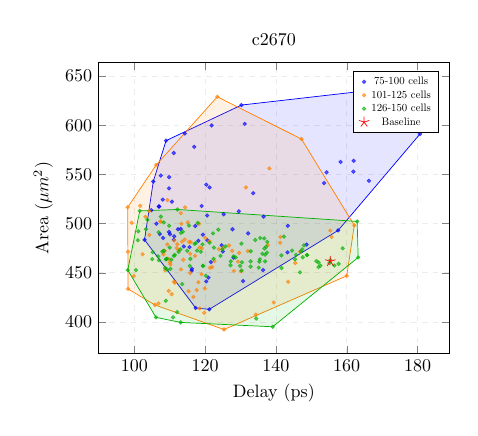
\begin{tikzpicture}[scale=0.65]
\begin{axis}[
    title={c2670},
    xlabel={Delay (ps)},
    ylabel={Area ($\mu m^2$)},
    legend pos=north east,
    legend style={nodes={scale=0.6, transform shape}},
    grid=both,
    grid style={dashed, opacity=0.3}
]
  \addplot [color=blue, fill=blue, fill opacity=0.1, forget plot] coordinates { (102.87, 483.59) (117.31, 414.31) (121.17, 412.91) (157.58, 493.15) (180.71, 591.13) (175.71, 639.19) (130.26, 620.52) (108.95, 584.37) (105.34, 542.84) (102.87, 483.59) };
  \addplot [color=orange, fill=orange, fill opacity=0.1, forget plot] coordinates { (106.17, 559.64) (98.12, 516.72) (98.20, 433.67) (105.81, 417.34) (125.32, 392.38) (160.01, 446.96) (162.14, 498.29) (147.21, 586.00) (123.43, 628.92) (106.17, 559.64) };
  \addplot [color=green!70!black, fill=green!70!black, fill opacity=0.1, forget plot] coordinates { (139.08, 395.18) (163.23, 465.63) (162.95, 502.25) (112.18, 514.38) (101.52, 512.98) (98.13, 452.80) (106.10, 404.74) (113.07, 399.61) (139.08, 395.18) };
  \addplot [only marks, mark=*, mark size=1pt, color=blue, opacity=0.6] coordinates { (143.27, 470.76) (112.33, 494.32) (120.31, 441.37) (166.28, 543.54) (148.65, 478.69) (121.84, 599.76) (124.65, 477.99) (121.17, 412.91) (161.96, 563.84) (105.34, 542.84) (109.80, 535.84) (158.26, 562.67) (125.22, 509.48) (175.71, 639.19) (127.72, 494.32) (114.27, 591.60) (107.47, 548.91) (130.71, 441.60) (120.33, 539.58) (119.00, 517.88) (132.14, 490.12) (153.60, 541.21) (116.25, 453.96) (125.02, 471.69) (111.25, 487.09) (109.79, 491.52) (136.51, 507.15) (113.97, 476.82) (111.15, 483.59) (154.31, 552.17) (161.87, 552.87) (130.26, 620.52) (109.81, 547.27) (107.19, 489.42) (121.63, 460.96) (120.64, 483.12) (133.58, 530.95) (110.07, 489.19) (108.02, 524.41) (180.71, 591.13) (118.08, 482.66) (106.94, 517.42) (116.19, 452.10) (106.95, 517.42) (111.12, 571.77) (110.60, 522.31) (120.95, 445.10) (116.91, 578.07) (120.55, 508.32) (143.35, 497.82) (102.87, 483.59) (131.18, 601.40) (108.11, 485.46) (128.01, 465.39) (108.95, 584.37) (136.36, 452.80) (157.58, 493.15) (129.50, 512.52) (106.24, 499.92) (121.24, 536.78) (104.79, 513.68) (117.31, 414.31) (115.57, 476.12) (113.09, 494.55) (119.37, 488.72) (117.21, 497.59) };
  \addlegendentry{75-100 cells}
  \addplot [only marks, mark=*, mark size=1pt, color=orange, opacity=0.6] coordinates { (109.34, 523.95) (115.30, 431.33) (120.04, 485.46) (115.75, 469.36) (115.11, 501.32) (118.46, 413.84) (126.73, 477.76) (98.20, 471.46) (138.13, 556.14) (147.21, 586.00) (131.53, 536.78) (146.81, 471.46) (113.27, 499.92) (115.78, 449.76) (106.17, 559.64) (111.17, 440.90) (103.13, 506.92) (117.12, 467.26) (111.95, 475.19) (118.99, 448.60) (123.43, 628.92) (119.08, 474.96) (119.89, 434.13) (114.32, 516.48) (121.35, 455.13) (155.35, 492.92) (113.81, 463.29) (115.47, 481.49) (108.24, 468.89) (145.45, 460.03) (112.13, 479.16) (111.25, 482.89) (110.53, 428.30) (109.28, 478.92) (118.07, 440.43) (110.18, 458.63) (109.76, 463.99) (113.44, 481.72) (141.19, 480.56) (143.46, 440.90) (128.12, 451.86) (139.40, 419.90) (113.13, 510.65) (107.54, 502.02) (130.08, 451.63) (125.32, 392.38) (114.22, 483.82) (134.32, 407.54) (102.33, 468.89) (105.81, 417.34) (117.61, 432.50) (111.47, 439.97) (108.58, 472.39) (119.75, 409.41) (98.12, 516.72) (129.60, 470.29) (107.29, 502.25) (99.85, 446.73) (115.92, 481.26) (106.80, 418.97) (113.16, 453.50) (123.85, 474.02) (162.14, 498.29) (116.69, 425.50) (101.63, 518.11) (98.20, 433.67) (124.97, 475.19) (118.26, 499.92) (110.04, 460.49) (160.01, 446.96) (109.69, 431.57) (118.44, 475.66) (104.17, 512.75) (104.24, 488.49) (122.63, 461.89) (137.69, 478.22) (121.99, 455.83) (108.66, 452.80) (99.24, 500.85) (141.25, 486.39) (127.64, 472.39) (112.45, 473.33) (132.04, 472.16) (121.21, 482.19) (129.28, 461.43) (155.74, 486.39) };
  \addlegendentry{101-125 cells}
  \addplot [only marks, mark=*, mark size=1pt, color=green!70!black, opacity=0.6] coordinates { (117.03, 479.39) (111.41, 468.19) (127.17, 457.70) (109.81, 497.82) (120.23, 446.96) (162.95, 502.25) (141.54, 467.73) (112.07, 410.11) (137.55, 481.49) (163.23, 465.63) (115.43, 498.05) (135.53, 485.46) (119.25, 478.92) (132.87, 471.93) (122.21, 490.12) (128.03, 466.79) (113.15, 490.59) (100.44, 452.80) (136.16, 469.36) (136.77, 474.72) (123.71, 493.85) (151.43, 461.89) (110.93, 404.74) (105.05, 463.99) (117.90, 500.62) (114.91, 472.39) (109.98, 475.66) (110.19, 453.96) (115.67, 457.00) (139.08, 395.18) (158.86, 474.96) (106.10, 404.74) (125.72, 476.82) (118.78, 471.46) (108.67, 455.13) (144.54, 472.63) (113.70, 491.75) (134.42, 403.57) (128.63, 465.63) (117.72, 472.63) (136.68, 484.99) (113.07, 399.61) (109.22, 464.46) (117.37, 480.32) (135.14, 455.36) (101.12, 492.22) (122.38, 464.23) (105.16, 470.99) (103.70, 503.88) (107.48, 507.15) (148.78, 468.19) (115.82, 464.23) (106.72, 466.79) (106.85, 491.29) (111.16, 467.26) (113.01, 473.79) (130.26, 479.62) (134.15, 483.36) (108.30, 501.32) (145.69, 468.19) (98.13, 452.80) (137.48, 470.53) (136.96, 468.43) (122.48, 475.66) (152.02, 455.83) (156.52, 457.46) (142.25, 486.86) (121.26, 480.56) (119.41, 457.00) (107.95, 471.69) (108.88, 421.54) (119.36, 457.23) (155.13, 460.03) (141.56, 454.90) (109.25, 453.26) (135.32, 461.43) (146.78, 450.46) (152.57, 457.23) (135.46, 463.76) (112.18, 514.38) (113.51, 438.57) (130.29, 452.33) (101.00, 483.12) (148.78, 467.96) (110.44, 463.29) (124.87, 473.79) (108.35, 472.39) (106.95, 462.83) (147.43, 473.79) (147.06, 471.69) (145.39, 463.76) (147.57, 465.86) (157.72, 459.10) (103.27, 494.32) (130.39, 460.73) (147.90, 477.99) (137.24, 476.59) (129.85, 457.00) (124.34, 467.26) (132.84, 461.66) (152.02, 460.49) (108.94, 463.76) (108.94, 463.76) (101.52, 512.98) (112.49, 471.23) (155.37, 463.06) (127.25, 461.66) (136.95, 461.66) (132.84, 456.30) };
  \addlegendentry{126-150 cells}
  \addplot [only marks, mark=star, mark size=3pt, color=red] coordinates { (155.37, 461.66) };
  \addlegendentry{Baseline}
\end{axis}
\end{tikzpicture}
\end{minipage}
\hfill
\begin{minipage}{0.32\textwidth}
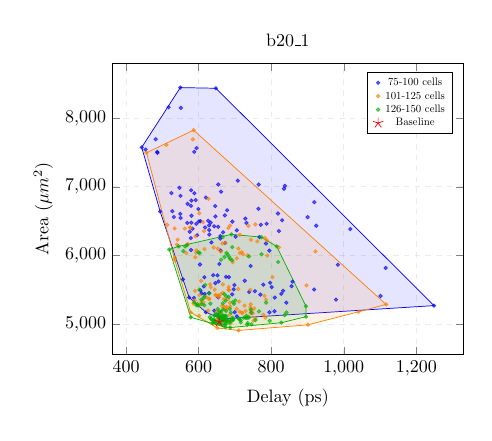
\begin{tikzpicture}[scale=0.65]
\begin{axis}[
    title={b20\_1},
    xlabel={Delay (ps)},
    ylabel={Area ($\mu m^2$)},
    legend pos=north east,
    legend style={nodes={scale=0.6, transform shape}},
    grid=both,
    grid style={dashed, opacity=0.3}
]
  \addplot [color=blue, fill=blue, fill opacity=0.1, forget plot] coordinates { (670.26, 5076.17) (1248.83, 5269.10) (647.73, 8435.41) (549.57, 8445.20) (443.26, 7574.37) (494.01, 6640.78) (557.00, 5650.27) (573.98, 5387.14) (620.18, 5172.28) (658.04, 5086.20) (670.26, 5076.17) };
  \addplot [color=orange, fill=orange, fill opacity=0.1, forget plot] coordinates { (586.21, 7825.61) (456.46, 7495.52) (534.07, 5938.61) (578.06, 5171.35) (651.68, 4943.67) (710.36, 4907.51) (901.34, 4988.93) (1041.11, 5179.28) (1116.83, 5286.12) (586.21, 7825.61) };
  \addplot [color=green!70!black, fill=green!70!black, fill opacity=0.1, forget plot] coordinates { (519.11, 6086.28) (578.49, 5098.57) (673.92, 4954.40) (687.06, 4949.27) (827.91, 5019.72) (896.14, 5107.43) (895.86, 5260.23) (815.21, 6132.23) (772.98, 6266.60) (690.35, 6306.96) (544.93, 6131.53) (519.11, 6086.28) };
  \addplot [only marks, mark=*, mark size=1pt, color=blue, opacity=0.6] coordinates { (620.18, 5172.28) (600.92, 6495.45) (739.40, 5468.55) (588.30, 6905.79) (578.65, 6252.84) (591.92, 6806.88) (764.89, 6679.74) (856.15, 5551.83) (629.04, 6369.48) (658.04, 5086.20) (835.33, 6971.34) (587.09, 5380.60) (527.60, 6644.98) (657.36, 5875.16) (549.40, 6605.79) (924.22, 6431.76) (547.27, 6985.34) (787.40, 6461.16) (708.20, 7089.15) (605.50, 6498.71) (810.15, 5385.97) (628.97, 6437.13) (801.34, 5539.00) (675.52, 5687.37) (661.88, 6929.12) (583.67, 6389.07) (617.02, 5440.32) (1248.83, 5269.10) (660.74, 6071.58) (633.21, 6477.95) (588.05, 7508.12) (647.73, 8435.41) (550.40, 6546.07) (646.14, 5596.39) (549.57, 8445.20) (818.78, 6611.16) (705.21, 6366.21) (517.45, 8159.43) (646.41, 6567.77) (481.71, 7692.87) (580.48, 6578.50) (765.59, 7032.93) (617.90, 6407.97) (575.62, 6344.52) (858.78, 5618.78) (580.31, 6799.65) (642.89, 6424.30) (525.08, 6908.35) (494.01, 6640.78) (550.28, 6867.76) (614.45, 5548.80) (672.47, 6583.40) (629.52, 6304.63) (832.83, 5485.81) (978.59, 5356.58) (731.98, 6473.29) (603.95, 5867.93) (595.87, 6294.13) (645.78, 6719.16) (771.46, 6445.76) (983.93, 5864.43) (830.17, 6513.18) (643.34, 5194.68) (654.10, 5391.10) (701.91, 6273.13) (579.46, 6950.11) (797.02, 5601.75) (620.29, 6843.04) (628.88, 5452.22) (837.69, 7013.56) (1017.97, 6384.17) (654.19, 7033.39) (593.68, 6460.92) (743.40, 5845.76) (531.91, 6560.53) (486.09, 7507.42) (608.40, 5448.25) (678.56, 6658.51) (767.66, 6267.30) (568.82, 6473.29) (770.20, 5429.13) (580.02, 6477.49) (755.33, 5479.28) (693.12, 6492.88) (778.25, 5573.76) (809.08, 5187.21) (599.35, 6676.01) (605.06, 5490.94) (551.20, 8149.64) (900.39, 6558.20) (1101.29, 5408.60) (918.83, 6776.08) (659.94, 6245.61) (640.21, 5712.33) (683.42, 5684.57) (579.03, 6079.51) (1115.66, 5818.24) (705.71, 5113.26) (795.01, 6069.95) (652.04, 5709.99) (626.48, 6504.78) (486.48, 7495.29) (569.72, 6750.66) (578.89, 6722.66) (727.21, 5630.91) (673.05, 6180.99) (692.66, 5433.56) (667.46, 6336.12) (453.83, 7542.41) (660.00, 6283.86) (653.95, 6416.83) (785.74, 6173.99) (635.35, 6189.38) (557.00, 5650.27) (654.99, 5620.88) (573.98, 5387.14) (670.26, 5076.17) (699.54, 5172.98) (918.46, 5503.54) (615.83, 5681.77) (841.78, 5311.55) (594.35, 7563.64) (696.61, 5506.57) (795.20, 5171.82) (728.62, 6537.21) (827.93, 5441.26) (698.67, 5568.63) (443.26, 7574.37) (653.52, 5134.96) (821.40, 6355.25) };
  \addlegendentry{75-100 cells}
  \addplot [only marks, mark=*, mark size=1pt, color=orange, opacity=0.6] coordinates { (743.41, 5171.58) (590.31, 5483.95) (570.34, 6165.36) (584.31, 7690.77) (921.91, 6058.28) (633.39, 5538.07) (566.02, 6032.85) (713.08, 5180.45) (691.62, 5066.38) (631.91, 5580.06) (456.46, 7495.52) (821.23, 6117.77) (586.21, 7825.61) (1041.11, 5179.28) (601.93, 6613.72) (578.06, 5171.35) (626.27, 5196.08) (677.22, 5224.77) (614.81, 6353.85) (644.33, 5501.68) (711.53, 5328.35) (803.68, 5684.80) (666.39, 5453.15) (513.47, 6446.93) (718.81, 6047.78) (649.65, 5060.54) (612.15, 6484.25) (577.12, 6404.70) (511.48, 7609.59) (686.61, 6435.03) (665.43, 6173.76) (590.75, 5972.90) (589.30, 5345.38) (710.36, 4907.51) (621.35, 5389.93) (612.48, 5319.48) (1116.83, 5286.12) (789.25, 5999.50) (534.40, 5965.67) (734.87, 6001.83) (591.11, 6278.73) (788.65, 6218.31) (686.31, 5139.39) (694.00, 5901.75) (901.34, 4988.93) (761.79, 6205.25) (653.18, 6099.57) (542.23, 6228.34) (648.15, 5419.09) (687.24, 5257.66) (785.77, 5356.34) (782.75, 6252.37) (682.23, 5500.51) (742.90, 5247.63) (704.90, 5221.74) (533.97, 6392.11) (686.17, 5310.62) (667.92, 5113.50) (709.33, 5511.47) (593.04, 6040.55) (743.73, 5288.22) (627.33, 6824.37) (654.92, 5416.53) (778.40, 5134.26) (682.97, 5541.57) (628.95, 5370.11) (670.88, 5250.90) (749.23, 5157.12) (753.12, 5228.04) (680.84, 5365.44) (641.83, 6115.67) (534.07, 5938.61) (688.54, 5014.59) (729.46, 5191.18) (661.35, 6055.72) (721.87, 6018.39) (781.67, 5411.16) (718.80, 5167.85) (745.87, 5194.91) (562.08, 6390.94) (897.36, 5564.19) (673.64, 5102.07) (742.63, 5499.81) (660.97, 5435.89) (721.16, 5159.92) (601.25, 5122.60) (602.14, 5422.83) (646.83, 5424.69) (651.68, 4943.67) (682.02, 6400.27) (671.43, 5212.88) (713.43, 6033.09) (650.69, 5182.78) (666.88, 5578.66) (673.79, 6184.72) (607.22, 5320.18) (705.32, 5958.20) (683.97, 5494.21) (744.30, 6227.88) (713.42, 6302.06) (655.75, 5391.10) (586.05, 5299.42) (540.41, 6158.13) (576.30, 6406.57) (681.61, 5038.85) (669.74, 5362.87) (784.22, 5090.87) (756.54, 6452.06) (709.70, 6099.81) (616.05, 6093.27) (629.68, 5364.97) (594.05, 6075.54) (603.05, 5276.09) (738.35, 5107.90) (657.36, 5098.57) (726.64, 5269.10) (660.09, 5165.52) (641.60, 5008.52) (664.69, 5265.36) (737.50, 6429.66) (677.63, 5251.37) (751.10, 5048.41) (756.25, 5087.37) (567.64, 6154.39) (606.93, 5629.28) };
  \addlegendentry{101-125 cells}
  \addplot [only marks, mark=*, mark size=1pt, color=green!70!black, opacity=0.6] coordinates { (676.28, 5044.68) (684.66, 5061.48) (632.61, 5298.02) (687.18, 5947.94) (785.99, 5312.72) (735.50, 5012.72) (683.21, 5395.53) (815.21, 6132.23) (658.70, 5011.79) (745.52, 5163.42) (618.19, 5569.56) (654.76, 5042.58) (689.16, 5040.01) (657.71, 5183.02) (661.80, 5085.27) (662.94, 5102.07) (630.96, 5102.07) (692.70, 5094.60) (694.99, 5058.91) (842.28, 5168.55) (836.96, 5130.06) (695.82, 5076.41) (676.60, 5404.16) (599.80, 6046.38) (603.23, 6033.09) (645.26, 5138.23) (766.39, 5184.41) (650.98, 5123.76) (738.59, 5093.67) (648.20, 5020.42) (634.91, 5075.24) (607.42, 5355.18) (772.98, 6266.60) (743.75, 5211.71) (773.25, 6017.22) (562.81, 6130.60) (578.49, 5098.57) (668.91, 5124.23) (652.85, 5221.27) (684.64, 5019.02) (668.60, 5074.54) (519.11, 6086.28) (895.86, 5260.23) (655.67, 5085.50) (670.90, 5436.82) (672.88, 4996.86) (674.59, 5048.88) (716.05, 5024.85) (544.93, 6131.53) (675.84, 5189.78) (687.06, 4949.27) (700.91, 5345.61) (666.70, 6267.77) (648.85, 5145.92) (613.12, 5376.17) (697.71, 5295.46) (557.96, 6062.48) (593.88, 5274.93) (667.10, 5302.69) (674.95, 5000.59) (738.68, 5985.50) (686.14, 5221.27) (692.73, 6120.57) (629.59, 5448.25) (680.21, 6010.46) (731.53, 5120.03) (677.21, 5114.43) (729.46, 5092.50) (615.83, 5273.76) (659.60, 5022.52) (674.42, 5340.01) (745.58, 4997.32) (587.75, 5317.85) (733.47, 5086.90) (670.40, 5031.85) (724.41, 5090.87) (666.14, 5064.98) (661.17, 5099.50) (678.50, 5049.35) (690.35, 6306.96) (568.44, 6150.19) (634.30, 5075.01) (819.09, 5904.55) (756.99, 5057.74) (672.72, 5121.20) (638.23, 5016.45) (661.48, 5177.18) (694.35, 5319.48) (713.03, 5071.51) (647.22, 5022.05) (659.12, 5006.42) (615.89, 5401.83) (598.82, 5269.10) (667.10, 5212.64) (715.91, 5054.71) (641.44, 5032.08) (602.26, 5500.74) (666.70, 5058.21) (671.47, 5976.87) (643.40, 5117.23) (827.91, 5019.72) (676.85, 6035.19) (643.70, 5058.91) (664.44, 5130.76) (661.58, 5058.21) (670.85, 5100.20) (642.75, 5043.98) (733.83, 4992.43) (596.46, 5292.19) (641.12, 5054.01) (710.35, 5078.97) (896.14, 5107.43) (655.90, 5121.66) (689.14, 5168.55) (795.75, 5046.31) (668.74, 5100.67) (667.97, 5055.88) (661.99, 5936.51) (692.19, 5930.44) (609.00, 5292.42) (684.74, 5976.40) (660.93, 5062.64) (673.92, 4954.40) (655.25, 5017.85) (665.93, 4985.43) };
  \addlegendentry{126-150 cells}
  \addplot [only marks, mark=star, mark size=3pt, color=red] coordinates { (656.76, 5034.18) };
  \addlegendentry{Baseline}
\end{axis}
\end{tikzpicture}
\end{minipage}
\caption{Area-Delay scatter plot for randomly sample of ASAP7 (7nm.lib)}
\label{fig:random_sample}
\end{figure}


\section*{Assignment 3 (40\%): Standing on the shoulders of MapTune}

基於 MapTune 的結果 $S_{MapTune}$，我透過執行數輪 First-Choice Local Search，也就是不停尋找當前最佳解的鄰居，一一嘗試是否能找到更好的解。如 \autoref{alg:local_search} 所示，鄰居即為將當前選擇 $S_{curr}$ 加入或移除一個 cell 之後的新集合，而為了確保 $|S_{new}| \leq |S_{MapTune}|$，若當前選擇數量已經達到上限，將不允許加入 cell，只允許移除。若該輪沒有找到更好的解，則選擇本輪相對最好的解作為下一輪的初始解。若連續 2 輪沒有找到更好的解則結束，設定為 2 輪的原因是: 令當前最佳解為 $S_{best}$，若本輪沒找到更好的解，則會選擇本輪相對好的解 $S_{best}'$ 進入第二輪，由於 $S_{best}$ 與 $S_{best}'$ 互為鄰居，若第二輪也沒有找到更好的解，則必定會選擇 $S_{best}$ 進入第三輪，如此將產生不必要的重複嘗試，因此 2 輪就足夠了。

\begin{center}
\captionof{algorithm}{First-Choice Local Search for Library Tuning}
\label{alg:local_search}
\hrule height.5pt depth0pt \kern4pt
\begin{algorithmic}[1]
\Require $\mathcal{F}$ (set of all available cells), $S_{MapTune}$ (initial selected cells from MapTune)
\State $S_{best} \gets S_{MapTune}, S_{curr} \gets S_{MapTune}$
\State $R_{best} \gets \text{CalculateReward}(S_{MapTune})$
\State $P_{no\_improv} \gets 0$ \Comment{Counter for consecutive non-improving rounds}

\While{$P_{no\_improv} < 2$}
    \State $R_{round} \gets -\infty$, $S_{round} \gets \emptyset$
    \State $found\_better \gets \textbf{false}$

    \For{each $c \in \mathcal{F}$}
        \If{$c \in S_{curr}$}
            \State $S_{sel} \gets S_{curr} \setminus \{c\}$ \Comment{Remove currently selected cell}
        \Else
            \If{$|S_{curr}| \geq |S_{MapTune}|$}
                \State \textbf{continue} \Comment{Skip adding if budget is reached}
            \EndIf
            \State $S_{sel} \gets S_{curr} \cup \{c\}$ \Comment{Add unselected cell}
        \EndIf

        \State $r \gets \text{CalculateReward}(S_{sel})$
        
        \If{$r > R_{round}$}
            \State $R_{round} \gets r, S_{round} \gets S_{sel}$
        \EndIf
        
        \If{$r > R_{best}$}
            \State $R_{best} \gets r, S_{best} \gets S_{sel}$
            \State $S_{curr} \gets S_{sel}$
            \State $P_{no\_improv} \gets 0$
            \State $found\_better \gets \textbf{true}$
            \State \textbf{break} \Comment{Accept the first better solution immediately}
        \EndIf
    \EndFor

    \If{\textbf{not} $found\_better$}
        \State $S_{curr} \gets S_{round}$ \Comment{Fallback to the best candidate in this round}
        \State $P_{no\_improv} \gets P_{no\_improv} + 1$
    \EndIf
\EndWhile

\State \textbf{return} $S_{best}, R_{best}$
\end{algorithmic}
\kern2pt\hrule\relax
\end{center}

以 c2670.bench + nan45.genlib 選擇 54 個 cells 為例，如下方執行結果所示，在 MapTune 完成 100 個 iteration，得到約 -0.873 的 reward 之後，我的程式成功找到了 7 次更好的解，最終將 reward 提升到了約 -0.858。其中 success 代表該輪找到了更好的解，fail 則否。

\begin{lstlisting}
$ python batched_MAB_EP.py 54 benchmarks/c2670.bench nan45.genlib
select 54 cells from 82 cells
keep 12 cells
Baseline Delay: 441.04
Baseline Area: 493.96
Batch iteration: 0
Current best reward:  -0.9626917908272263
Current best result:  (440.53, 458.32)
Batch iteration: 1
Current best reward:  -0.9626917908272263
Current best result:  (440.53, 458.32)
Batch iteration: 2
Current best reward:  -0.8862500973818875
Current best result:  (366.33, 467.1)

...

Batch iteration: 99
Current best reward:  -0.8726437910806986
Current best result:  (359.47, 461.51)
Best Delay: 359.47
Best Area: 461.51
Best Reward: -0.8726437910806986
Total time: 111.19865918159485
  1: success, best reward: -0.8692, delay: 355.85, area: 462.57, cells count: 53
  2: success, best reward: -0.8671, delay: 359.29, area: 455.92, cells count: 54
  3: success, best reward: -0.8664, delay: 354.78, area: 460.98, cells count: 53
  4: success, best reward: -0.8651, delay: 353.51, area: 461.24, cells count: 52
  5: success, best reward: -0.8602, delay: 349.11, area: 461.78, cells count: 53
  6: success, best reward: -0.8600, delay: 348.12, area: 462.84, cells count: 52
  7: success, best reward: -0.8584, delay: 350.25, area: 458.32, cells count: 51
  8: fail, round best reward: -0.8584, delay: 350.25, area: 458.32, cells count: 52
  9: fail, round best reward: -0.8584, delay: 350.25, area: 458.32, cells count: 51
Best Reward: -0.8583977999741299
Best Delay: 350.25
Best Area: 458.32
Best Cells Count: 51
Total time: 149.6730215549469
\end{lstlisting}

\autoref{tab:optimization_results} 是對 s13207、c2670、b20\_1 分別使用 nan45、sky130 在 budgets 為 30\%、50\%、70\% 時，MapTune (batched\_MAB\_EP) 與我的方法的結果比較，可以發現我的方法成功達成了 $S_{new} \le S_{MapTune}$ 且 $ADP_{new} < ADP_{MapTune}$ 的目標。

然而從執行時間可以發現，此方法仍然不太穩定，有些 case 比 MapTune 快上許多，但有些卻花了 MapTune 3 倍以上的時間執行。且 Local Search 並不能保證找到更優解，有可能在一開始就連續 2 輪失敗導致結束，因此未來或許可以嘗試加入了溫度的 Simulated Annealing，使其跳脫 Local Maximum 以找到更好的解。

\begin{table*}[htbp]
\centering
\caption{Performance Comparison between MapTune and Proposed Local Search}
\resizebox{\textwidth}{!}{
\begin{tabular}{llc|rrrrr|rrrrr}
\toprule
\multirow{2}{*}{\textbf{Benchmark}} & \multirow{2}{*}{\textbf{Library}} & \multirow{2}{*}{\textbf{Budget}} & \multicolumn{5}{c|}{\textbf{MapTune}} & \multicolumn{5}{c}{\textbf{Proposed Method}} \\
\cmidrule(lr){4-8} \cmidrule(l){9-13}
& & & Delay (ps) & Area ($\mu m^2$) & Reward & $|S_{MapTune}|$ & Time(s) & Delay (ps) & Area ($\mu m^2$) & Reward & $|S_{new}|$ & Time(s) \\
\midrule
b20\_1       & nan45        & 30\% & 1223.85 & 7726.50 & -0.9513 & 16   & 532.91 & 1162.30 & 7399.85 & -0.9073 & 16   & 197.27 \\
             &              & 50\% & 1434.47 & 7103.26 & -0.9875 & 35   & 981.76 & 1400.69 & 6910.68 & -0.9625 & 34   & 223.59 \\
             &              & 70\% & 1402.04 & 6978.24 & -0.9677 & 54   & 488.13 & 1336.58 & 7014.15 & -0.9473 & 54   & 236.90 \\
\midrule
b20\_1       & sky130       & 30\% & 6392.30 & 36999.23 & -1.0273 & 85   & 659.37 & 5735.84 & 36318.58 & -0.9641 & 85   & 1099.80 \\
             &              & 50\% & 6286.38 & 35713.00 & -1.0009 & 154  & 679.09 & 5962.02 & 35630.42 & -0.9736 & 154  & 1021.78 \\
             &              & 70\% & 6147.25 & 34779.61 & -0.9767 & 222  & 713.05 & 5611.83 & 34501.84 & -0.9295 & 221  & 1478.92 \\
\midrule
c2670        & nan45        & 30\% & 365.24 & 513.38 & -0.9277 & 16   & 110.36 & 352.58 & 444.49 & -0.8482 & 16   & 46.70 \\
             &              & 50\% & 367.25 & 458.05 & -0.8787 & 35   & 112.98 & 365.83 & 450.07 & -0.8694 & 35   & 20.00 \\
             &              & 70\% & 359.47 & 461.51 & -0.8726 & 54   & 111.20 & 350.25 & 458.32 & -0.8584 & 51   & 38.47 \\
\midrule
c2670        & sky130       & 30\% & 1709.33 & 2448.60 & -0.9748 & 85   & 184.36 & 1446.96 & 2398.55 & -0.8877 & 84   & 196.47 \\
             &              & 50\% & 1751.06 & 2253.41 & -0.9465 & 154  & 186.22 & 1421.07 & 2223.38 & -0.8470 & 154  & 359.68 \\
             &              & 70\% & 1781.76 & 2312.22 & -0.9672 & 222  & 206.09 & 1512.49 & 2232.14 & -0.8755 & 221  & 287.58 \\
\midrule
s13207       & nan45        & 30\% & 576.02 & 2220.04 & -0.9728 & 16   & 175.45 & 522.57 & 2107.25 & -0.9027 & 16   & 111.30 \\
             &              & 50\% & 593.88 & 2033.84 & -0.9454 & 35   & 175.74 & 558.39 & 2006.44 & -0.9105 & 34   & 77.79 \\
             &              & 70\% & 578.15 & 1992.34 & -0.9232 & 54   & 164.28 & 551.34 & 1986.49 & -0.9002 & 53   & 47.54 \\
\midrule
s13207       & sky130       & 30\% & 2874.09 & 11091.89 & -0.9701 & 85   & 262.23 & 2594.86 & 11065.61 & -0.9207 & 83   & 736.86 \\
             &              & 50\% & 2753.67 & 10625.19 & -0.9294 & 154  & 276.75 & 2536.92 & 10721.53 & -0.8961 & 153  & 739.71 \\
             &              & 70\% & 2705.81 & 10854.16 & -0.9311 & 222  & 279.45 & 2616.68 & 10866.67 & -0.9162 & 213  & 969.61 \\
\bottomrule
\end{tabular}
}
\label{tab:optimization_results}
\end{table*}


\section*{Conclusion}

本次作業透過 MapTune 框架探討了 partial library 對於邏輯合成中 PPA 的影響。實驗結果不僅驗證了縮減後的元件庫能帶來更佳的 Area-Delay Product (ADP)，我所嘗試的 First-Choice Local Search 演算法也成功在各個 benchmark 與 budget 限制下，穩定超越了原本 MapTune 的基準測試結果，同時嚴格滿足了 $|S_{new}| \le |S_{MapTune}|$ 的條件限制。

雖然 Greedy 策略在執行時間上存在較大波動，且容易陷入局部最佳解，但整體而言，本實驗充分展示了自動化 Library Tuning 在 EDA 領域的巨大潛力。未來若能結合 Simulated Annealing 等更進階的啟發式演算法，預期能進一步提升優化穩定度與探索空間。

\section*{Source Code}

完整實驗用到的程式碼可以在 \url{https://github.com/co0okie/NTUST-Logic-Synthesis-and-Verification-PA3-MapTune} 找到。

\end{document}